\documentclass[10pt]{article}
\usepackage{amsmath}
\usepackage{tikz}
\usepackage{enumerate}
\usepackage[margin=1in]{geometry}
\usepackage{graphicx}
\usepackage{amsmath}
\graphicspath{{../../Screenshots/}}
\usetikzlibrary{arrows.meta, positioning}
\begin{document}
\section{Determining mass action law}
Given reaction:
$$aA+bB\leftrightarrow cC+dD$$
\begin{center}
    \begin{tabular}{|c|c|}
        \hline
        molar quantity &$\frac{\Delta G}{n} = \Delta\bar{G}$
        \\\hline
        partial molar quantity & $ \frac{\partial\Delta G}{\partial n} = \mu$
        \\\hline
    \end{tabular}
\end{center}
Gibbs free energy:
$$dG = -SdT + VdP + \sum \mu_idn_i$$
for a constant Temperature and Pressure process:
$$dG = \sum \mu_idn_i$$
$$\mu_adn_A+\mu_bdn_B=\mu_cdn_C+\mu_ddn_D$$
Assuming A, B, C, and D are all pure, $\Delta \bar{G} = \mu$
$$\bar{G}_i=\bar{G}_i^\circ + RT \ln P_i = \mu_i$$
\begin{align*}
    n_A(G^\circ+RT \ln P)_A +  n_B(G^\circ+RT \ln P)_B &=  n_C(G^\circ+RT \ln P)_C +  n_D(G^\circ+RT \ln P)_D
    \\
    G_{\text{tot}}^\circ = \sum n_i G_i^\circ =
    n_A \bar{G}^\circ_A + n_B \bar{G}^\circ_B + n_C \bar{G}^\circ_C + n_D \bar{G}^\circ_D &= 
    (nRT \ln P)_A + (nRT \ln P)_B - (nRT \ln P)_C - (nRT \ln P)_D
    \\
    G_{\text{tot}}^\circ &= RT \ln(\frac{P_A^{n_A}P_B^{n_B}}{P_C^{n_C}P_D^{n_D}})
    \\
    &= -RT \ln(\frac{P_C^{n_C}P_D^{n_D}}{P_A^{n_A}P_B^{n_B}}) 
    \\
     &= -RT \ln(k) 
\end{align*}
\section{Solid-gas reaction (Phase equilibria)}
consider oxidation(two components):
$$M_{(s)}+1/2O_{2(g)} \leftrightarrow MO_{(s)}$$
\begin{center}
    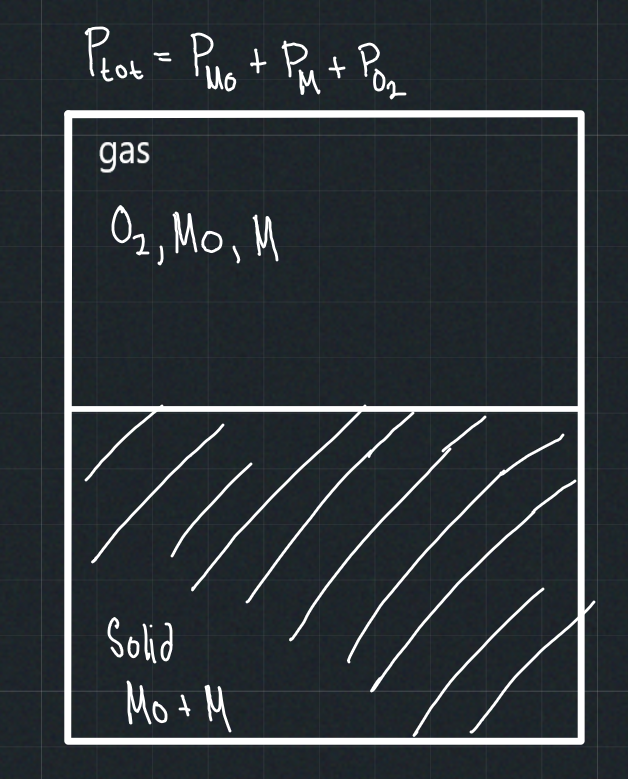
\includegraphics[width = 200pt]{Screenshot 2025-11-28 121816.png}
\end{center}
\begin{align*}
   \Delta \bar{G_i} &= \Delta G_i^\circ + RT \ln P_i
   \\
   \mu_i 
   &= \mu_i^\circ + RT \ln P_i 
   \\
   G_{\text{tot}}^\circ &= \sum n_i G_i^\circ = \sum \mu_i dn_i 
   = G^\circ_{(s)}
\end{align*}
\end{document}
